\section{Introduction and Motivation}

When faster hardware can no longer be created by just adding more
logic, engineers have to look for more energy efficient solutions
in order to keep power density down. Current research consists of
many branches reaching from homogeneous processors to heterogeneous
systems with loads of interconnect.

\begin{figure}
\begin{subfigure}[b]{0.48\textwidth}
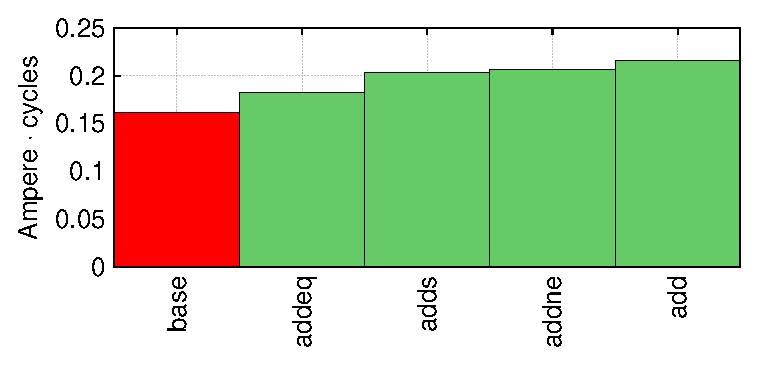
\includegraphics[width=\textwidth]{graph_01_base_cond-0c6.eps}
\caption{Conditional execution (eq is false).}
\end{subfigure}
\begin{subfigure}[b]{0.52\textwidth}
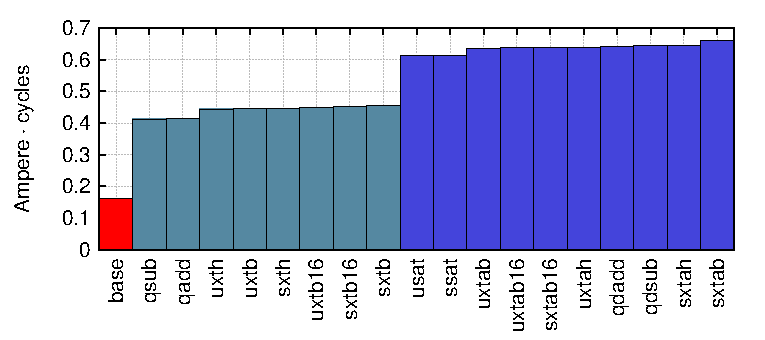
\includegraphics[width=\textwidth]{graph_023_base_quad_saturate_extend-0c6.eps}
\caption{Non-multiply multi-cycle instructions.}
\end{subfigure}
\caption{Figures from \cite{rundehvatum2013exploring} showing the results of measuring the
current drain through the CPU core while running isolated instructions in a loop.}
\end{figure}

